\def\notedate{2023.01.25}
\def\currentauthor{Журавлев Н.В. (РК6-72Б)}
\notestatement{rndhpcedt}{Разработка архитектуры программной реализации}

В реализации программы должны быть реализованы четыре главных сценария действия: Открыть из файла, создание графа, сохранение в файлы, найти цикл. Так же необходимо создать простую базу данных для хранения графов для каждого пользователя. Общий вид схемы модулей представлен на рисунке \ref{fig:module}. В программе должно быть реализована 2 класса - Graph (класс графа) и Node (класс вершина). 

\begin{figure}[h]
    \centering
    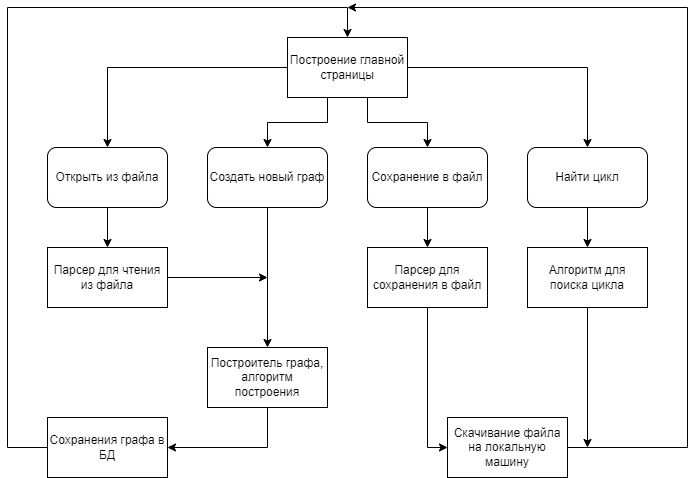
\includegraphics[width=0.7\linewidth]{ResearchNotes/rndhpc_int_edt_2023_01_25/module.png}
    \caption{Схема модулей программы}
    \label{fig:module}
\end{figure} 

В классе узла должны иметься следующий поля: словарь с ключом в виде следующих узлов и код при переходе к следующему узлу, являющимся значением являющейся строкой; название для узла.

Краткое описание модулей и их взаимодействия:
\begin{itemize}
\item Открыть из файла - модуль , для этого необходимо реализовать алгоритм укладки графа и парсер для преобразования из файла типа aDot в массив объектов класса узла.
\item Создать новый граф - модуль ответственный за добавление/удаление частей графа с помощью ручного ввода.
\item Сохранение в файл - модуль ответственный за сохранения графа в файл типа aDot, для этого необходимо реализовать парсер для преобразования в нужный форма из массива объектов класса узла.
\item Найти цикл - модуль ответственный за нахождение цикла в графе, для этого необходимо реализовать алгоритм поиска цикла в графе.
\end{itemize}

В классе графа в полях должно иметься массив класса узлов, в методах должны быть реализованы:
\begin{itemize}
\item make_graph(name) - метод, которые преобразует массив в объекте класса в переменную, которую можно сохранить в виде изображения с выбранным расширением.
\item read_from_aDot(name) - метод, читающей из файла с названием name (тип string) данные, затем сохраняет их в поле для узлов. 
\item search_cicles() - метод, который находит циклы в графе, возвращает все циклы в виде строки формата "a-b-c[перенос строки]b-d-e[перенос строки]".
\item add_eage(e1, e2) - метод, добавляющий ребро между двумя узлами из e1 (тип класса узла) в e2 (тип класса узла)
\item delete_eage(e1, e2) - метод, удаляющий ребро между двумя узлами из e1 (тип класса узла) в e2 (тип класса узла)
\item add_node(node) - метод, добавляет узел node.
\item delete_node(node) - метод, удаляющий узел node.
\item save_into_aDot(name) - метод, сохраняет граф в файл с названием name (тип string)
\end{itemize}

В базе данных необходимо иметь одну таблицу с двумя полями: пользователь и его граф в текстовом виде.

\noteattributes{}